% GNUPLOT: LaTeX picture with Postscript
\begingroup
  \makeatletter
  \providecommand\color[2][]{%
    \GenericError{(gnuplot) \space\space\space\@spaces}{%
      Package color not loaded in conjunction with
      terminal option `colourtext'%
    }{See the gnuplot documentation for explanation.%
    }{Either use 'blacktext' in gnuplot or load the package
      color.sty in LaTeX.}%
    \renewcommand\color[2][]{}%
  }%
  \providecommand\includegraphics[2][]{%
    \GenericError{(gnuplot) \space\space\space\@spaces}{%
      Package graphicx or graphics not loaded%
    }{See the gnuplot documentation for explanation.%
    }{The gnuplot epslatex terminal needs graphicx.sty or graphics.sty.}%
    \renewcommand\includegraphics[2][]{}%
  }%
  \providecommand\rotatebox[2]{#2}%
  \@ifundefined{ifGPcolor}{%
    \newif\ifGPcolor
    \GPcolortrue
  }{}%
  \@ifundefined{ifGPblacktext}{%
    \newif\ifGPblacktext
    \GPblacktexttrue
  }{}%
  % define a \g@addto@macro without @ in the name:
  \let\gplgaddtomacro\g@addto@macro
  % define empty templates for all commands taking text:
  \gdef\gplbacktext{}%
  \gdef\gplfronttext{}%
  \makeatother
  \ifGPblacktext
    % no textcolor at all
    \def\colorrgb#1{}%
    \def\colorgray#1{}%
  \else
    % gray or color?
    \ifGPcolor
      \def\colorrgb#1{\color[rgb]{#1}}%
      \def\colorgray#1{\color[gray]{#1}}%
      \expandafter\def\csname LTw\endcsname{\color{white}}%
      \expandafter\def\csname LTb\endcsname{\color{black}}%
      \expandafter\def\csname LTa\endcsname{\color{black}}%
      \expandafter\def\csname LT0\endcsname{\color[rgb]{1,0,0}}%
      \expandafter\def\csname LT1\endcsname{\color[rgb]{0,1,0}}%
      \expandafter\def\csname LT2\endcsname{\color[rgb]{0,0,1}}%
      \expandafter\def\csname LT3\endcsname{\color[rgb]{1,0,1}}%
      \expandafter\def\csname LT4\endcsname{\color[rgb]{0,1,1}}%
      \expandafter\def\csname LT5\endcsname{\color[rgb]{1,1,0}}%
      \expandafter\def\csname LT6\endcsname{\color[rgb]{0,0,0}}%
      \expandafter\def\csname LT7\endcsname{\color[rgb]{1,0.3,0}}%
      \expandafter\def\csname LT8\endcsname{\color[rgb]{0.5,0.5,0.5}}%
    \else
      % gray
      \def\colorrgb#1{\color{black}}%
      \def\colorgray#1{\color[gray]{#1}}%
      \expandafter\def\csname LTw\endcsname{\color{white}}%
      \expandafter\def\csname LTb\endcsname{\color{black}}%
      \expandafter\def\csname LTa\endcsname{\color{black}}%
      \expandafter\def\csname LT0\endcsname{\color{black}}%
      \expandafter\def\csname LT1\endcsname{\color{black}}%
      \expandafter\def\csname LT2\endcsname{\color{black}}%
      \expandafter\def\csname LT3\endcsname{\color{black}}%
      \expandafter\def\csname LT4\endcsname{\color{black}}%
      \expandafter\def\csname LT5\endcsname{\color{black}}%
      \expandafter\def\csname LT6\endcsname{\color{black}}%
      \expandafter\def\csname LT7\endcsname{\color{black}}%
      \expandafter\def\csname LT8\endcsname{\color{black}}%
    \fi
  \fi
    \setlength{\unitlength}{0.0500bp}%
    \ifx\gptboxheight\undefined%
      \newlength{\gptboxheight}%
      \newlength{\gptboxwidth}%
      \newsavebox{\gptboxtext}%
    \fi%
    \setlength{\fboxrule}{0.5pt}%
    \setlength{\fboxsep}{1pt}%
    \definecolor{tbcol}{rgb}{1,1,1}%
\begin{picture}(3740.00,4020.00)%
    \gplgaddtomacro\gplbacktext{%
    }%
    \gplgaddtomacro\gplfronttext{%
      \csname LTb\endcsname%%
      \put(206,613){\makebox(0,0)[r]{\strut{}}}%
      \csname LTb\endcsname%%
      \put(206,959){\makebox(0,0)[r]{\strut{}}}%
      \csname LTb\endcsname%%
      \put(206,1306){\makebox(0,0)[r]{\strut{}}}%
      \csname LTb\endcsname%%
      \put(206,1653){\makebox(0,0)[r]{\strut{}}}%
      \csname LTb\endcsname%%
      \put(206,2000){\makebox(0,0)[r]{\strut{}}}%
      \csname LTb\endcsname%%
      \put(206,2346){\makebox(0,0)[r]{\strut{}}}%
      \csname LTb\endcsname%%
      \put(206,2693){\makebox(0,0)[r]{\strut{}}}%
      \csname LTb\endcsname%%
      \put(206,3040){\makebox(0,0)[r]{\strut{}}}%
      \csname LTb\endcsname%%
      \put(206,3386){\makebox(0,0)[r]{\strut{}}}%
      \csname LTb\endcsname%%
      \put(304,263){\makebox(0,0){\strut{}$-180$}}%
      \csname LTb\endcsname%%
      \put(824,263){\makebox(0,0){\strut{}$-120$}}%
      \csname LTb\endcsname%%
      \put(1344,263){\makebox(0,0){\strut{}$-60$}}%
      \csname LTb\endcsname%%
      \put(1864,263){\makebox(0,0){\strut{}$0$}}%
      \csname LTb\endcsname%%
      \put(2384,263){\makebox(0,0){\strut{}$60$}}%
      \csname LTb\endcsname%%
      \put(2904,263){\makebox(0,0){\strut{}$120$}}%
      \csname LTb\endcsname%%
      \put(3425,263){\makebox(0,0){\strut{}$180$}}%
      \csname LTb\endcsname%%
      \put(1864,0){\makebox(0,0){\normalsize $\Phi$}}%
      \csname LTb\endcsname%%
      \put(2113,1669){\rotatebox{-34.00}{\makebox(0,0){\strut{}\textcolor{black}{\footnotesize 9}}}}%
      \csname LTb\endcsname%%
      \put(2479,616){\rotatebox{-22.00}{\makebox(0,0){\strut{}\textcolor{black}{\footnotesize 9}}}}%
      \csname LTb\endcsname%%
      \put(2227,1010){\rotatebox{69.00}{\makebox(0,0){\strut{}\textcolor{black}{\footnotesize 6}}}}%
      \csname LTb\endcsname%%
      \put(2087,2015){\rotatebox{-38.00}{\makebox(0,0){\strut{}\textcolor{black}{\footnotesize 6}}}}%
      \csname LTb\endcsname%%
      \put(2794,535){\rotatebox{-151.00}{\makebox(0,0){\strut{}\textcolor{black}{\footnotesize 6}}}}%
      \csname LTb\endcsname%%
      \put(1386,3024){\rotatebox{39.00}{\makebox(0,0){\strut{}\textcolor{black}{\footnotesize 3}}}}%
      \csname LTb\endcsname%%
      \put(2164,1208){\rotatebox{70.00}{\makebox(0,0){\strut{}\textcolor{black}{\footnotesize 3}}}}%
      \csname LTb\endcsname%%
      \put(2101,2097){\rotatebox{-39.00}{\makebox(0,0){\strut{}\textcolor{black}{\footnotesize 3}}}}%
      \csname LTb\endcsname%%
      \put(3015,568){\rotatebox{-131.00}{\makebox(0,0){\strut{}\textcolor{black}{\footnotesize 3}}}}%
      \csname LTb\endcsname%%
      \put(2718,3465){\rotatebox{24.00}{\makebox(0,0){\strut{}\textcolor{black}{\footnotesize 3}}}}%
      \csname LTb\endcsname%%
      \put(1694,3339){\rotatebox{91.00}{\makebox(0,0){\strut{}\textcolor{black}{\footnotesize 1}}}}%
      \csname LTb\endcsname%%
      \put(2826,3439){\rotatebox{28.00}{\makebox(0,0){\strut{}\textcolor{black}{\footnotesize 1}}}}%
      \csname LTb\endcsname%%
      \put(1909,1511){\rotatebox{128.00}{\makebox(0,0){\strut{}\textcolor{black}{\footnotesize 1}}}}%
      \csname LTb\endcsname%%
      \put(2180,2110){\rotatebox{-34.00}{\makebox(0,0){\strut{}\textcolor{black}{\footnotesize 1}}}}%
      \csname LTb\endcsname%%
      \put(3124,597){\rotatebox{-116.00}{\makebox(0,0){\strut{}\textcolor{black}{\footnotesize 1}}}}%
      \csname LTb\endcsname%%
      \put(1864,3823){\makebox(0,0){DBA EA (meV)}}%
    }%
    \gplbacktext
    \put(0,0){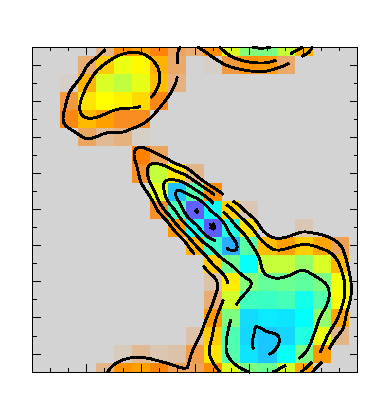
\includegraphics[width={187.00bp},height={201.00bp}]{Q1_DBA}}%
    \gplfronttext
  \end{picture}%
\endgroup
